\documentclass[PianoDiQualifica.tex]{subfiles}

\begin{document}
%http://www.praxiom.com/iso-90003.htm citato da Tullio può servire come base per capire processi meglio
\chapter{Qualità di processo}

\section{Scopo} 
Per garantire la qualità del prodotto è necessario perseguire la qualità dei processi che lo definiscono.
Per raggiungere questo obiettivo, si è deciso di seguire il principio di miglioramento continuo (\citGloss{PDCA}) e di adottare lo standard ISO/IEC 15504 denominato SPICE (Software Process Improvement and Capability Determination).

\section{Procedure di controllo di qualità di processo}
La qualità dei processi verrà garantita dall'applicazione del metodo \citGloss{PDCA}, descritto dell'appendice A. Grazie a questo metodo sarà possibile ottenere un miglioramento continuo della qualità di tutti i processi, inclusa la \citGloss{verifica}, e come diretta conseguenza si otterrà il miglioramento dei prodotti risultanti. 

Per ottenere qualità dei processi, bisogna:
\begin{itemize}
	\item \textbf{Definire il processo}: affinché sia controllabile;
	\item \textbf{Controllare il processo}: in funzione dell'ottenimento di efficacia, efficienza ed esperienza;
	\item \textbf{Usare strumenti di valutazione}: SPICE e \citGloss{PDCA}.
\end{itemize}

\section{Processi}

\subsection{Pianificazione di progetto, impostazione e controllo di processi}
Il macro-processo ha lo scopo di produrre dei piani di sviluppo per il progetto, comprendenti la scelta del modello di ciclo di vita del prodotto, descrizioni delle attività e dei compiti da svolgere, pianificazione temporale del lavoro e dei costi da sostenere, allocazione di compiti e responsabilità e misurazioni per rilevare lo stato del progetto rispetto alle pianificazioni prodotte.

\subsubsection{Obbiettivi}
Lo sviluppo del progetto dovrà porre particolare attenzione a rispettare dei particolari obbiettivi:
\begin{itemize}
	\item \textbf{Budget:} utilizzando le metriche descritte nella sezione seguente, si deve tenere sempre controllato l'utilizzo del budget, al fine di non avere scarti eccessivi con il costo preventivato;
	\item \textbf{Task:} porre attenzione alla pianificazione dei task e al loro completamento, assicurandosi che seguano la metodologia del miglioramento continuo, affinché tutti i compiti ne traggano vantaggio;
	\item \textbf{Educazione personale:} avere accortezza che ogni membro del gruppo abbia un livello di preparazione adatto all'esecuzione dei task assegnati, al fine di evitare ritardi sul calendario;
	\item \textbf{Calendario:} assicurare una pianificazione adatta ai compiti da svolgere, per evitare scostamenti dal budget preventivato;
	\item \textbf{Standard:} definire standard di processo ogni qualvolta sia possibile, per facilitare il lavoro in gruppo e favorire un incremento continuo.
\end{itemize}

\subsubsection{Strategie}
Ogni eventuale valore negativo a livello di Schedule o Budget Variance rilevato sarà compensato con la revisione delle attività da svolgere e i \citGloss{requisiti} da ottenere, per valutare se nei tempi di calendario stabiliti la pianificazione sia corretta o se sia necessario rivedere la programmazione.\\
Il controllo verrà favorito con strumenti come \citGloss{Asana} e i diagrammi di \citGloss{Gantt} in modo tale da verificare l'andamento del progetto, per avere sempre una visione chiara e quantificabile del lavoro in corso affinché il lavoro non subisca ritardi.\\
Saranno sempre presenti delle finestre di \citGloss{Slack} per evitare sovrapposizioni di task dovute a eventuali ritardi o imprevisti. 

\subsubsection{Metriche} 
\paragraph{}
\textlink{MPS001TAB}{MPS001}{\textbf{MPS001 Schedule Variance (SV)}}\\
Indica se si è in linea, in anticipo o in ritardo, rispetto alla schedulazione delle attività di progetto pianificate nella \citGloss{baseline}.\\
È un indicatore di efficacia soprattutto nei confronti del Cliente. \\
Se il valore SV ottenuto è positivo significa che il progetto sta procedendo con una maggiore velocità rispetto a quanto pianificato, viceversa se negativo.\\
\textbf{Misurazione:}
\begin{center}
	 $ SV = BCWP – BCWS $
\end{center}
Dove: \begin{itemize}
	\item \textbf{BCWP (Budgeted Cost of Work Performed)}: è il valore (in giorni o Euro) delle attività realizzate alla data corrente.
	Rappresenta il valore prodotto dal progetto ossia il valore dei deliverable rilasciati fino al momento della misurazione in seguito alle attività svolte;
	\item \textbf{BCWS (Budgeted Cost of Work Scheduled)}: è il costo pianificato (in giorni o Euro) per realizzare le attività di progetto alla data corrente.
\end{itemize}


\paragraph{}
\textlink{MPS002TAB}{MPS002}{\textbf{MPS002 Budget Variance (BV)}}\\
Indica se alla data corrente si è speso di più o di meno rispetto a quanto previsto a budget alla data corrente.\\
È un indicatore che ha un valore unicamente contabile e finanziario.\\
Se il valore BV ottenuto è positivo significa che il progetto sta spendendo il proprio budget con minor velocità di quanto pianificato, viceversa se negativo.\\

\textbf{Misurazione:}
\begin{center}
	$ BV = BCWS – ACWP $
\end{center}
Dove: \begin{itemize}
	\item \textbf{BCWS (Budgeted Cost of Work Scheduled)}: è il costo pianificato (in giorni o Euro) per realizzare le attività di progetto alla data corrente;
	\item \textbf{ACWP (Actual Cost of Work Performed)}: è il costo effettivamente sostenuto (in giorni o Euro) alla data corrente.
\end{itemize}


\subsection{Verifica software}
Il processo punta a verificare se qualsiasi elemento del sistema soddisfa completamente i \citGloss{requisiti} ad esso assegnati.
\subsubsection{Obiettivi}
Per poter definire delle \citGloss{baseline} per lo sviluppo del software, è necessario che il codice venga sempre verificato.
 \begin{itemize}
 	\item \textbf{Commenti al codice:} ogni unità di codice dovrà essere sufficientemente commentata affinché sia ritenuta verificabile;
 	\item \textbf{Prevenzione di bug:} accertarsi per quanto possibile che ogni unità di codice non sia affetta da bug prima dell'utilizzo.
 \end{itemize}
\subsubsection{Strategie}
Per prevenire bug e vulnerabilità al codice si utilizzano strumenti come Sonarlint e Sonarqube al fine di evitare la propagazione di errori ed avere una panoramica sullo stato generale del codice prodotto.\\
Si utilizzeranno delle metriche di Code Coverage per avere consapevolezza della quantità di codice testato e poter agire di conseguenza.
 
\subsubsection{Metriche}
\paragraph{Code Coverage}
Per poter avere una misura di codice testato e verificato si adoreranno determinati coverage criteria:
\begin{itemize}
	\item \textlink{MPS003TAB}{MPS003}{\textbf{MPS003 Function coverage:}} verificare che ogni funzione sia stata chiamata;
	\item \textlink{MPS004TAB}{MPS004}{\textbf{MPS004 Statement coverage:}} verificare che ogni statement del codice sia stato eseguito; 
	\item \textlink{MPS005TAB}{MPS004}{\textbf{MPS005 Branch coverage:}} verificare se tutti i possibili branch (derivanti da if e case statement) sono stati eseguiti;
	\item \textlink{MPS006TAB}{MPS006}{\textbf{MPS006 Condition coverage:}} verificare se ogni condizione booleana è stata valutata sia nella condizione true che false. 
\end{itemize}

\textbf{Misurazione:}
Vengono calcolate in percentuale sulla quantità di codice testato e verificato oltre che sul totale delle linee di codice scritte, tramite tool automatici come IstanbulJS\footnote{\nURI{https://istanbul.js.org/}}.


\section{Tabella delle metriche}
% ID METRICA
% M --> metrica
% PS--> processo
% (lettera per macro categoria, se esistono)
% 00n --> numero incrementale
Questa tabella indica i \textbf{range} di accettazione e di ottimalità per le metriche utilizzate per la qualità di processo:
\begin{table}[H]
	\begin{center}
		\begin{tabu} to \textwidth {
				>{\centering}m{0.1\linewidth}
				>{\centering}m{0.4\linewidth}
				>{\centering}m{0.2\linewidth} 
				>{\centering\arraybackslash}m{0.2\linewidth}
			}
			\tableHeaderStyle
			
			\textbf{ID} & \textbf{Nome} & \textbf{Range di accettazione} & \textbf{Range di ottimalità}\\
			\textlink{MPS001}{MPS001TAB}{MPS001} & Schedule Variance & $ \geq -5\% $ & $ \geq 0 $ \\
			\textlink{MPS002}{MPS002TAB}{MPS002} & Budget Variance & $ \geq -10\% $ & $ \geq 0 $ \\
			\textlink{MPS003}{MPS003TAB}{MPS003} & Function coverage & $ \geq 98\% $ & $ 100\% $\\
			\textlink{MPS004}{MPS004TAB}{MPS004} & Statement coverage &  $ \geq 97\% $& $ 100\% $\\
			\textlink{MPS005}{MPS005TAB}{MPS005} & \citGloss{branch} coverage & $ \geq 95\% $ & $ 100\% $\\
			\textlink{MPS006}{MPS006TAB}{MPS006} & Condition coverage & $ \geq 99\% $ & $ 100\% $\\ % lasciate questo capo riga


		\end{tabu}
		\caption{Tabella delle metriche della qualità di processo}
		\vspace{-1em}
	\end{center}
\end{table}




\begin{appendices}

\chapter{Ciclo di Deming o PDCA}
Ogni processo deve essere organizzato basandosi sul principio del miglioramento continuo (o \citGloss{ciclo di Deming}):
\begin{description}
	\item [Plan (pianificare)]: viene definito un piano che basandosi sulla definizione di problemi e obiettivi pianifica compiti, assegna responsabilità, studia il caso, analizza le cause della criticità e definisce azioni correttive; 
	\item [Do (eseguire)]: vengono implementate le attività secondo le linee definite durante la fase Plan;
	\item [Check (valutare)]: viene verificato l'esito delle azioni di miglioramento rispetto alle attese;
	\item [Act (agire)]: vengono applicate le correzioni necessarie per colmare le carenze rilevate e vengono standardizzate le attività correttamente eseguite.
\end{description}

\begin{figure}[htbp]
	\begin{center}
		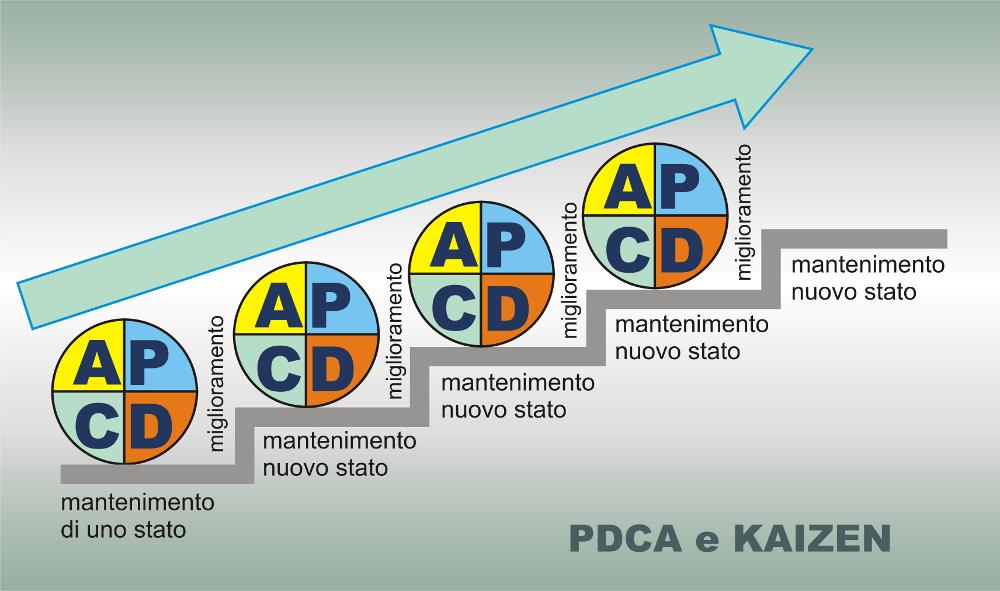
\includegraphics[width=0.7\linewidth]{PDCAkaizen}
		\caption[Ciclo di Deming]{Ciclo di Deming}
		\label{fig:pdca}
	\end{center}
\end{figure}

\chapter{ISO/IEC 15504}
Lo standard ISO/IEC 15504 contiene un modello di riferimento che definisce 
\begin{itemize}
	\item Process dimension;
	\item Capability dimension.
\end{itemize}

La dimensione di processo divide i processi in cinque categorie:
\begin{itemize}
	\item Customer-supplier;
	\item Engineering;
	\item Supporting;
	\item Management;
	\item Organization.
\end{itemize}

Per ogni processo, lo standard ISO/IEC 15504 definisce dei livelli di capacità:
\begin{description}
	\item [\normalfont Livello 5] \textbf{Optimizing process}: il processo è continuamente migliorato;
	\item [\normalfont Livello 4] \textbf{Predictable process}: il processo è adottato sistematicamente, entro limiti definiti;
	\item [\normalfont Livello 3] \textbf{Established process}: un processo stabilito si basa su un processo standard;
	\item [\normalfont Livello 2] \textbf{Managed process}: il processo è gestito e i prodotti sono stabiliti, controllati e mantenuti;
	\item [\normalfont Livello 1] \textbf{Performed process}: il processo è implementato e raggiunge lo scopo stabilito;
	\item [\normalfont Livello 0] \textbf{Incomplete process}: il processo non è implementato o non raggiunge lo scopo stabilito.\\
\end{description}

La capacità dei processi viene misurata attraverso degli attributi di processo.
\begin{itemize}
\item Livello 1
	\begin{itemize}
		 \item \textbf{Process performance:} capacità di un processo di raggiungere gli obiettivi trasformando input identificabili in output identificabili;
	\end{itemize}
\item Livello 2
	\begin{itemize}
		 \item \textbf{Performance management:} capacità del processo di elaborare un prodotto coerente con gli obiettivi fissati;
		\item \textbf{Work product management:} capacità del processo di elaborare un prodotto documentato, controllato e verificato;
	\end{itemize}
\item Livello 3
	\begin{itemize}
		\item \textbf{Process definition:} l'esecuzione del processo si basa su standard di processo per raggiungere i propri obiettivi;
		\item \textbf{Process deployment:} capacità del processo di attingere a risorse tecniche e umane appropriate per essere attuato efficacemente;
	\end{itemize}
\item Livello 4
	\begin{itemize}
		 \item \textbf{Process measurement:} gli obiettivi e le misure di prodotto e di processo vengono usati per garantire il raggiungimento dei traguardi definiti in supporto ai target aziendali;
		\item \textbf{Process control:} il processo viene controllato tramite misure di prodotto e processo per effettuare correzioni migliorative al processo stesso;
	\end{itemize}
\item Livello 5
	\begin{itemize}
		 \item \textbf{Process innovation:} i cambiamenti strutturali, di gestione e di esecuzione vengono gestiti in modo controllato per raggiungere i risultati fissati;
		\item \textbf{Process optimization:} le modifiche al processo sono identificate e implementate per garantire il miglioramento continuo nella realizzazione degli obiettivi di business dell'organizzazione. 
	\end{itemize}
\end{itemize}

Ogni attributo consiste di una o più pratiche generiche che sono ulteriormente elaborate in indicatori pratici per aiutare la valutazione delle performance, sotto forma di indici N-P-L-F:
\begin{itemize}
	\item Non soddisfatto (0 - 15\%);
	\item Parzialmente soddisfatto ($ > $15\% - 50\%);
	\item Largamente soddisfatto ($ > $50\% - 85\%);
	\item Totalmente soddisfatto ($ > $85\% - 100\%)
\end{itemize}

\end{appendices}
\end{document}